\documentclass[main.tex]{subfiles}

\begin{document}

\section{V-Model}

The V-Model is a unique, linear development methodology, defined by the late Paul Rook in the 1980s, used during a software development life cycle.
It was accepted in Europe and UK as a progressive alternative to the Waterfall model.

The V-Model focuses on fairly typical waterfall-esque method that follows strict, step-by-step stages. While initial stages are broad design stages, progress proceeds down through more and more granular stages, leading into implementation and coding, and finally back through all testing stages prior to completion of the project.

\subsection{The Process of V-Model}

\begin{wrapfigure}[13]{l}[2em]{0.6\textwidth}
	\vspace*{-\baselineskip}
	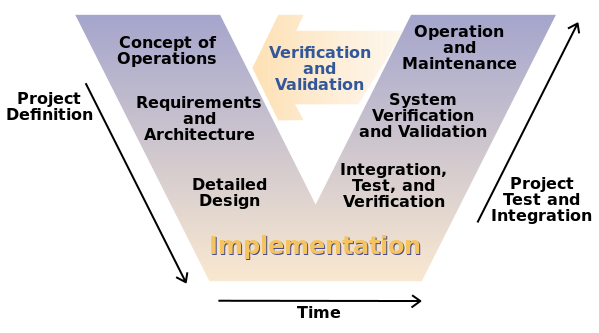
\includegraphics[scale=0.42]{vmodel-v.png}
	\caption{The V-Model stages\label{fig:vmodel-v}}
\end{wrapfigure}

Much like the traditional waterfall model, the V-Model specifies a series of linear stages that should occur across the life cycle, one at a time, until the project is complete.
For this reason, V-Model is not considered an agile development method, and due to the sheer volume of stages and their integration into the overall process, understanding the model in detail can be challenging for everyone on the team, let alone the client or users.

The V-shape of the V-Model represents the various stages that will be passed through during the software development lifecycle.
Beginning at the top-left stage and working, over time, toward the top-right tip, the stages represent a linear progression of development rather similar to the waterfall model.

So V-Model contains Verification phases on the left and Validation phases on the right of the development phase --- hence the name.

\subsubsection{Design Phase}

\paragraph{Requirements Gathering and Analysis}
Contains detailed communication with the customer to understand the requirements and their expectations.

\paragraph{System Design}
Contains the system design and the complete hardware and communication setup for developing the product.

\paragraph{Architectural Design}
System design is broken down further into modules taking up different functionality. The data transfer and communication between the internal modules and with the outside world (other systems) is clearly understood.

\paragraph{Module or Low-Level Design} Here the detailed design of each module is specified.

\subsubsection{Testing Phases}

\paragraph{Unit Testing}
Unit Test Plans are developed during the module design phase. These Unit Test Plans are executed to eliminate simple bugs at code or unit level.

\paragraph{Integration testing}
After completion of unit testing come integration tests, which verify the communication of modules among themselves.

\paragraph{System Testing}
Tests the application as whole, including functionality, interdependency and communication.

\paragraph{User Acceptance Testing (UAT)}
UAT is performed in a user environment that resembles the production environment. It verifies that the delivered system meets the user’s requirements and is ready for use in real time.

\subsection{Advantages of V-Model}

\paragraph{Suited for Restricted Projects}
Due to the stringent nature of the V-Model and its linear design, implementation, and testing phases, it's perhaps no wonder that V-Model has been heavily adopted by the medical device industry in recent years.
In situations where the project length and scope are well-defined and limited, the technology is stable, and the documentation and design specifications are clear and constant, then this will be a great method.

\paragraph{Ideal for Time Management}
Along the same vein, V-Model is also well-suited for projects that must maintain a strict deadline and meet key milestone dates throughout the process.
With fairly clear and well-understood stages that the whole team can easily comprehend and prepare for, it is relatively simple to create a timeline for the entire development lifecycle, while generating milestones for each stage along the way. Of course, V-Model in no way ensures milestones will always be met, but the strict nature of the model itself enforces the need to keep to a fairly right schedule.

\subsection{Disadvantages of V-Model}

\paragraph{Lacks Adaptability}
Similar to the issues facing the traditional waterfall model on which the V-Model is based, the most problematic aspect is the inability to adapt to any necessary changes during the development lifecycle.
For example, an overlooked issue within some fundamental system design, that is then only discovered during the implementation phase, can present a severe setback in terms of lost man-hours as well as increased costs.

\paragraph{Timeline Restrictions}
While not an inherent problem with the V-Model itself, the focus on testing at the end of the life cycle means that it’s all too easy to be pigeonholed at the end of the project into performing tests in a rushed manner to meet a particular deadline or milestone.

\paragraph{Ill-Suited for Lengthy Life Cycles}
Like the waterfall model, the V-Model is completely linear, and thus projects cannot be easily altered once the development train has left the station.
V-Model is therefore poorly suited to handle long-term projects that may require many versions or constant updates/patches.

\paragraph{Encourages ‘Design-by-Committee’ Development}
While V-Model is certainly not the only development model to fall under this criticism, it cannot be denied that the strict and methodical nature of the V-Model and its various linear stages tend to emphasize a development cycle befitting managers and users, rather than developers and designers.
It can be all too easy for project managers or others to overlook the vast complexities of software development in favor of trying to meet deadlines or to simply feel overly confident in the process or current progress, based solely on what stage in the life cycle is actively being developed.

\nocite{*}

\end{document}